\chapter{Background}
\label{cha:background}
The Stratosphere is a layer of the Earth's atmosphere characterised by increasing temperatures with height. This feature distinguishes it from the lowest layer of the atmosphere, the troposphere, and makes it stable to vertical convection. As a result, the stratosphere exhibits significantly different dynamical behaviour to the troposphere. The stratosphere is bounded by the tropopause from below and the stratopause above. The height of these bounds vary latitudinally with tropopause heights ranging from  xxx at the equator to $\sim$ xxx km in the polar regions. While the stratosphere and troposphere are characterised seperately, current understanding of atmospheric dynamics incorporates elements of coupling between the layers. This chapter outlines the key points of this current understanding including dynamics of the polar and equatorial stratosphere, stratosphere-troposphere coupling as well as surface variability relevant to the stratosphere.


\section{The Stratospheric Polar Vortex}
\label{sec:polar_vortex}
During Northern Hemisphere (NH) winter, the NH polar stratosphere is plunged into polar night. As a result, it experiences a net cooling effect through emission of longwave infrared radiation to space and the absence of shortwave solar radiation available for absorption. This significant cooling increases the meridional temperature gradient between the polar region and the tropics. This causes an increase in the vertical shear of zonal wind according to the thermal wind balance relation,

\begin{equation} \label{eq:thermal_wind}
\frac{\partial u_g}{\partial z} = -\frac{R}{f H}\frac{\partial T}{\partial y},
\end{equation}

where $u_g$ is the geostrophic zonal wind velocity (the wind resulting in a balance between Coriolis and pressure gradient forces), $z$ is the height coordinate, $R$ is the specific gas constant and $H$ is the atmospheric scale height, the gain in altitude which leads to a reduction in atmospheric pressure by a factor of $e$ given by $H = RT_r/g$ (g = acceleration d due to gravity and $T_r$ is a reference temperature). $f$ in equation \ref{eq:thermal_wind} is the Coriolis parameter under a beta plane approximation which is given by

\begin{equation} \label{eq:beta_plane_approx}
f = f_0 + \beta y = 2 \Omega sin(\phi_0) + 2 \Omega cos(\phi_0)\frac{ y}{a},
\end{equation}

where $\phi_0$ is a reference latitude, $\Omega$ is the rotation rate of the earth and $a$ is the Earth's radius. This increase in vertical shear in $u_g$ leads to a strong, stratospheric, westerly flow circumnavigating the North Pole during boreal winter months. This feature is known as the northern hemisphere polar vortex or polar night jet. Henceforth we refer to it as the vortex.

The vortex contains a core of cold polar air in which temperatures can drop to around 200K in the lower stratosphere according to the European Centre for Medium Range Weather Forecasting (ECMWF) interim reanalysis data set (referred to as ERA-interim). Wintertime averaged zonal wind speeds are found to reach up to approximately $40ms^{-1}$ at the 10hPa level at a latitude of 60N. Figure \ref{fig:ERAclimDJF} shows the climatological zonal mean zonal wind (ZMZW) from ERA-interim for the December-February period. It exhibits the traits set out above with a persistent zonal westerly wind above the 30hPa level. The troposphere exhibits 2 westerly jets which show greatest magnitude winds at approximately xxx hPa. Also included in figure \ref{fig:ERAclimDJF} is the seasonal cycle in daily winds at 60N on the 10hPa level (near the edge of the vortex). On average, the vortex forms in mid xxxx and breaks down to be replaced with summer easterlies in xxx. These winds show a large degree of variability across different seasons (figure \ref{fig:ERAclimDJF} grey lines) with some seasons exhibiting anomalously strong westerly flow and others even exhibiting easterlies for a portion of the season. These effects are due to the action of atmospheric waves on the vortex and are described fully in the following section. 


\begin{figure}[h!]
\centering
    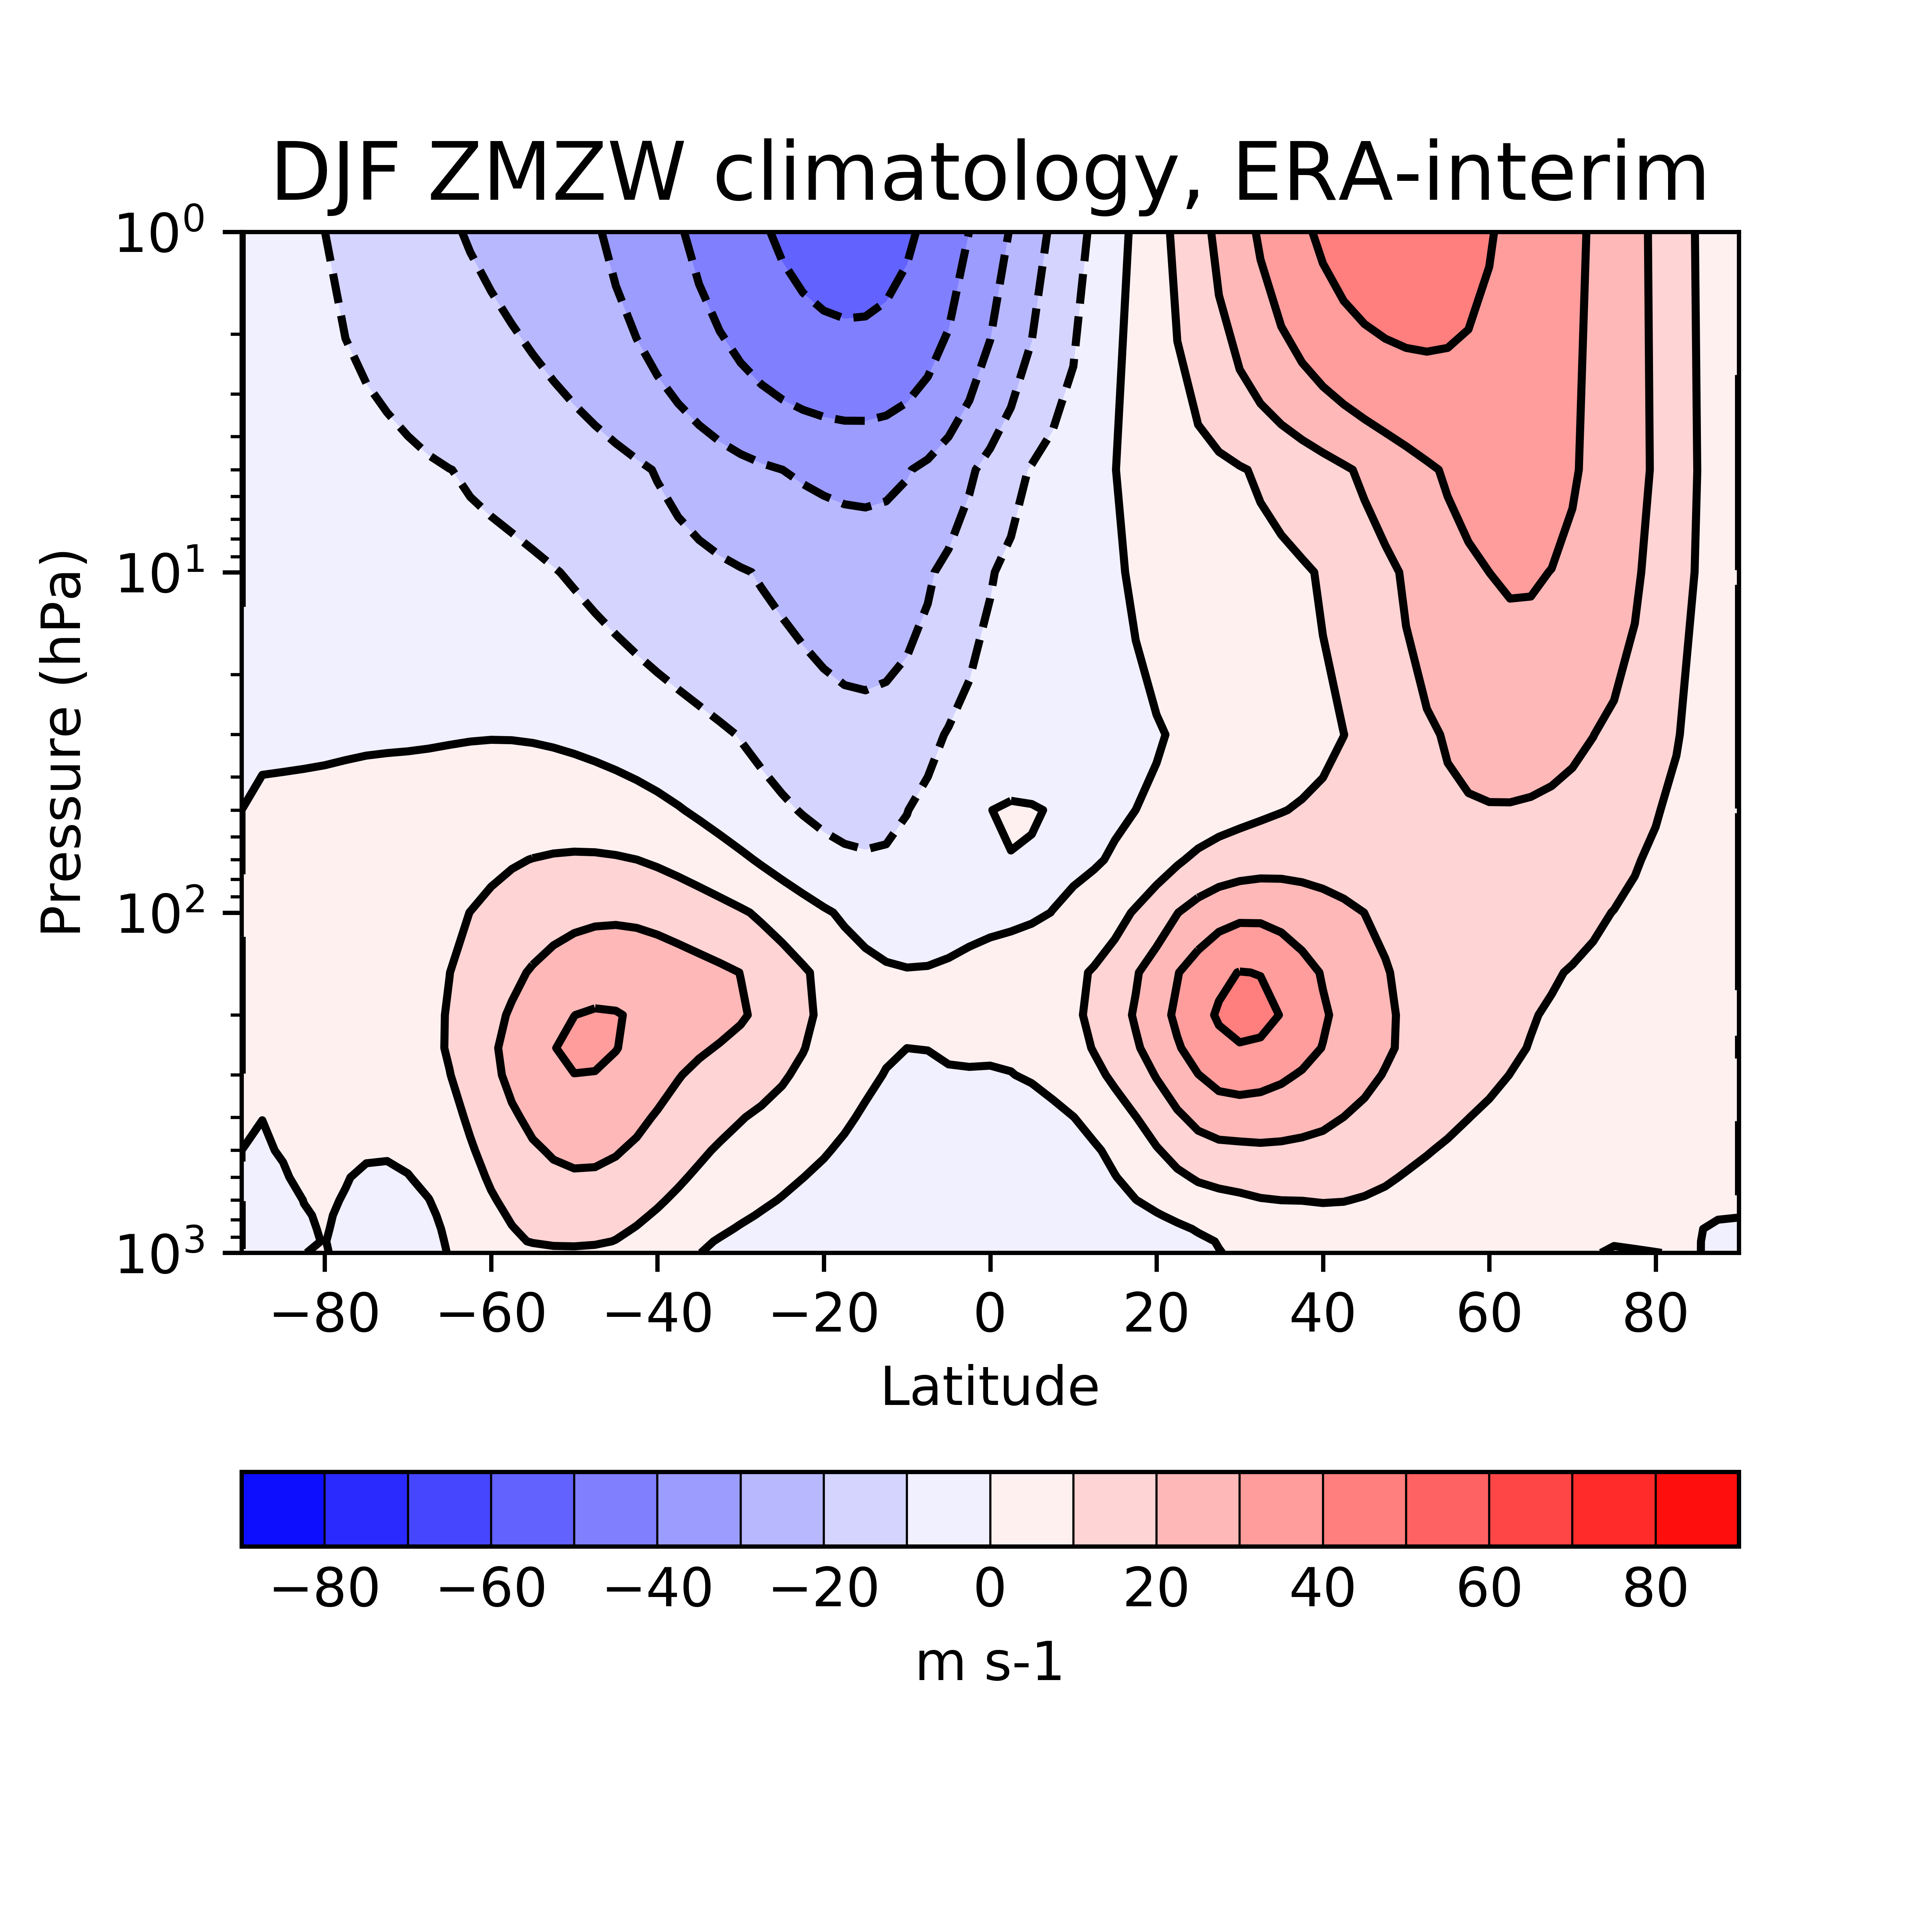
\includegraphics[width= 9cm]{Figures/Figures-background/fig1_for_transfer.png}
    \caption{DJF climatological zonal mean zonal wind from ERA-interim dataset between 1979 and 2018.}
    \label{fig:ERAclimDJF}
\centering
\end{figure}

\section{Atmospheric Waves}
\label{sec:atmos_waves}
Atmospheric wave is the term generally used for deviations from the zonal mean dynamical state and these phenomena, often referred to as Rossby waves, play a key role in the variability of the vortex. These waves are forced in the troposphere by air flowing over variations in topography (orographic waves) or through other mechanisms such as interaction with convection fronts and latent heat release (non-orographic). Perturbations originating near the surface can propagate vertically into the stratosphere altering large scale circulation features via wave drag as they transfer momentum to the background flow. 

Large scale Rossby waves are known as planetary waves and exhibit wavelengths of the order of $1000km$. The propagation of these waves can be described using the Quasi Geostrophic approximation for fluid in hydrostatic balance with low Rossby number, $R_0 = U/f_0 L$, where U and L are characteristic length and zonal velocity scales respectively. Under this framework the Quasi Geostrophic Potential Vorticity (QGPV) equation states that in the absence of friction and diabatic heating, the quasi geostrophic potential vorticity, $q$, is conserved following the geostrophic wind:

\begin{equation} \label{eq-PV_conserved}
D_g q = 0
\end{equation}

where $D_g$ is the operator 

\begin{equation}\label{eq:D_g}
D_g = \frac{\partial}{\partial t} + u_g \frac{\partial}{\partial x} + v_g\frac{\partial}{\partial y} 
\end{equation}

and $q$ can be written in terms of the stream function, $\psi$, in the QGPV framework as

\begin{equation} \label{eq:QGPV}
q = f_0 + \beta y + \nabla^2 \psi + \frac{\partial}{\partial z}\bigg(\frac{f_0^2}{N_B^2} \frac{\partial \psi}{\partial z}\bigg)
\end{equation}

where $N_B$ is the Brunt–Väisälä frequency, the frequency of vertical motion of a parcel of air in a stable atmosphere. $\psi$ is related to $u_g$ and $v_g$, the zonal and meridional components of geostrophic wind by $u_g = -\frac{\partial \psi}{\partial y}$ and $v_g = -\frac{\partial \psi}{\partial x}$. Under a further approximation of small disturbances from a uniform zonal flow, U, $\psi$ is given by

\begin{equation} \label{eq:Zonal_flow_SF}
\psi = -U y + \psi '
\end{equation}

where $\psi'$ is the contribution to the stream function from the small deviation from $U$. This approximation allows equation \ref{eq:QGPV} to be linearised to

\begin{equation} \label{eq:Linearised_QGPV}
\bigg(\frac{\partial}{\partial t} + U \frac{\partial}{\partial x}\bigg)\Gamma \psi' + \beta \frac{\partial \psi'}{\partial x} = 0,
\end{equation}

where $\Gamma$ is the operator

\begin{equation} \label{eq:ellipse_operator}
\Gamma = \nabla^2 \psi + \frac{\partial}{\partial z}\bigg(\frac{f_0^2}{N_B^2}\frac{\partial}{\partial z}\bigg).
\end{equation}

It can be shown that this equation has wave like solutions whose vertical propagation is only supported under the condition

\begin{equation} \label{eq:propagation_critera}
U - c = \frac{\beta k}{k^2 + l^2 + \frac{f_0^2 m^2}{N_B^2}} < U_c = \frac{\beta k}{k^2 + l^2}
\end{equation}

Where $U_c$ is a critical velocity corresponding to the background flow when $m = 0$, $c$ is the phase speed and $k, l$ and $m$ are the meridional, zonal and vertical wavenumbers of the wave respectively. Also imposing that, as $m^2 > 0$, $U - c > 0$ as well as assuming stationary waves ($c = 0$) gives 

\begin{equation} \label{eq:Charney-Drazin}
0 < U < U_c,
\end{equation}

the Charney-Drazin criterion for the vertical propagation of planetary waves. This result implies that vertical propagation can only occur through background westerly zonal flow with a magnitude less than some critical value, $U_c$, which depends on the horizontal wavenumbers of the wave. More specifically, equation \ref{eq:propagation_critera} shows that smaller wave-numbers (larger wavelengths) favours greater propagation and is the reason the majority of wave-mean flow interactions involving the vortex occur with disturbances of wavenumbers 1-3 (referred to as wave-n disturbances). 

\section{Sudden Stratospheric Warmings}

\subsection{The Equatorial Stratosphere}
\subsection{Stratosphere-Troposphere Coupling and Surface Variability}
\subsection{Stratosphere-Ocean Interactions}


